% D bar -> K 3pi feynman diagram
\RequirePackage{luatex85}

\documentclass{standalone}

\usepackage{tikz-feynman}

\begin{document}

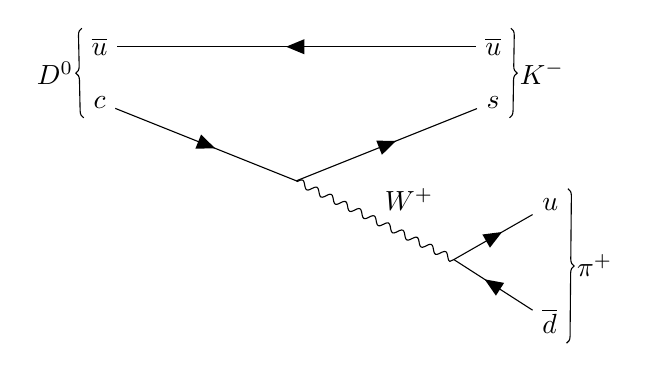
\begin{tikzpicture}
    \begin{feynman}
        \vertex (uBarIn) {\(\overline{u}\)};
        \vertex[right=5cm of uBarIn] (uBarOut) {\(\overline{u}\)};
        \vertex[below=2em of uBarIn] (c) {\(c\)};
        \vertex[right=5cm of c] (s) {\(s\)};
        \vertex[below right=1cm and 2.5cm of c] (v1);
        \vertex[below right=1cm and 2cm of v1] (v2);
        \vertex[above right=0.5cm and 1cm of v2] (u) {\(u\)};
        \vertex[below right=0.5cm and 1cm of v2] (dBar) {\(\overline{d}\)};
        \diagram* { {[edges=fermion]
                (uBarOut) -- (uBarIn),
                (c) -- (v1) -- (s), (dBar) -- (v2) -- (u)},
        (v1) -- [boson, edge label=\(W^+\)] (v2)
        };
        \draw [decoration={brace}, decorate] (c.south west) -- (uBarIn.north west) node [pos=0.5, left] {\(D^0\)};
        \draw [decoration={brace}, decorate] (uBarOut.north east) --  (s.south east) node [pos=0.5, right] {\(K^-\)};
        \draw [decoration={brace}, decorate] (u.north east) --  (dBar.south east) node [pos=0.5, right] {\(\pi^+\)};
    \end{feynman}
\end{tikzpicture}

\end{document}
